
\section{Prepare data}
\label{sec:dataPrepare}
In this section, we will introduce how to prepare gene expression data matrix as well as the clinical data files for the MetaOmics software suite.

\subsection{Raw data}

Gene expression matrix should be prepared as the example in Figure~\ref{fig:dataMicroarray}, saved in tab-delimited ``.txt" or comma-separated ``.csv" files.
The first column corresponds to the feature ID (e.g. gene symbol, probe id or entrez ID) and the rest of columns are the expression data from all the samples.
The first row contains the sample ID.
Valid data types include continuous data (e.g. those from microarray or FPKM data from RNA-seq) and count data (e.g. those from RNA-seq).

\begin{figure}[H]
\begin{center}
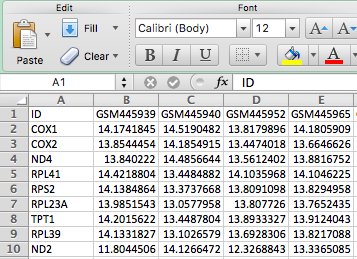
\includegraphics[scale=0.5]{./figure/dataPreparation/dataMicroarray}
\caption{A example input data format}
\label{fig:dataMicroarray}
\end{center}
\end{figure}

\subsection{Clinical data}

Clinical data should be prepared as the example in Figure~\ref{fig:clinical}.
The first column corresponds to the sample ID and the rest of columns contain the clinical information of the samples (e.g. case/control labels). Sample IDs of the clinical data (on rows) should be ordered in the same way as the gene expression data (on columns) to avoid any mismatch issues.  

\begin{figure}[H]
\begin{center}
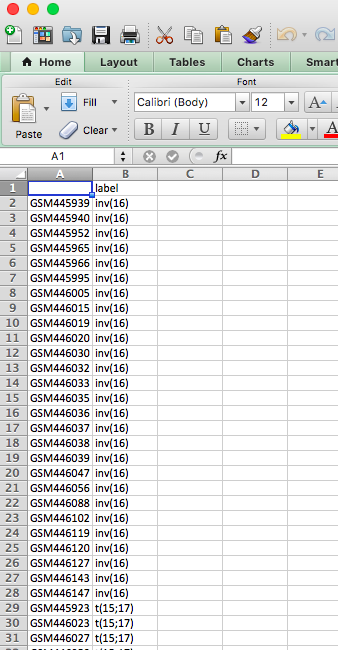
\includegraphics[scale=0.5]{./figure/dataPreparation/clinicalData}
\caption{A example clinical data format}
\label{fig:clinical}
\end{center}
\end{figure}

\subsection{Example data in the MetaOmics software}


We collected three multi-study data as the example datasets for the MetaOmics software.
Table~\ref{tab:realDataLeukemia} summarizes the first example dataset including three studies on acute myeloid leukemia (AML).
Table~\ref{tab:realDataBreastCancer} summarizes the second example dataset including four studies on breast cancer, where the first study contains both count data and FPKM data (continuous).
Table~\ref{tab:realDataProstate} summarizes the example dataset including eight studies on prostate cancer.
The leukemia data is used to demonstrate MetaPreprocess, MetaDE, MetaPath, MetaNetwork, MetaPredict, MetaClust and MetaPCA.
The prostate cancer data is used to demonstrate MetaQC.


			\begin{table}[H]
			\caption{Multi-study acute myeloid leukemia (AML) gene expression profiles. All three studies are from Affymetrix Human Genome U133plus2 with 5,135 genes.
		Three subtypes of leukemia are defined as the chromosomal translocation,
		including inversion of chromosome 16 - inv(16), translocation of chromosome 15 and 17 - t(15:17) and 
		translocation of chromosome 8 and 21 - t(8:21).}						
			\centering
\begin{tabular}{c  c  c   c   }
  \hline 
  \hline 
\multirow{2}*{Study}   & \multirow{2}*{source}   & \multirow{2}*{\# samples}  & \# samples by subtypes \\
 & & & inv(16)/t(15:17)/t(8,21)  \\
  \hline 
Study 1 & \cite{verhaak2009prediction} & 89 & 33/21/35\\
Study 2 & \cite{balgobind2011evaluation} & 74 & 27/19/28\\
Study 3 & \cite{kohlmann2008international} & 105 & 28/37/40\\
  \hline 
  \hline 
\end{tabular}
			\label{tab:realDataLeukemia}
		\end{table}
		
			\begin{table}[H]
			\caption{Multi-study breast cancer gene expression profiles. 
			Each gene expression profiles of all four studies contain 10,330 genes.
			Study 1 contains both count data and FPKM (continuous) data so user should {\bf select only one of them}. 
			The other three studies contain only continuous data.
			The phenotype of interest is estrogen-receptor (comparing ER+ vs ER-).}						
			\centering
			\begin{tabular}{c  c  c   c  c  }
			  \hline 
			  \hline 
			\multirow{2}*{Study}   & \multirow{2}*{source}   & \multirow{2}*{scale}  & \multirow{2}*{\# samples}  & \# samples by ER \\
 & & & & ER+/ER-  \\
  \hline 
\multirow{2}*{Study 1}  & \multirow{2}*{\cite{weinstein2013cancer}}  & count & \multirow{2}*{406} & \multirow{2}*{319/87}\\
&& continuous && \\
Study 2 & \cite{desmedt2007strong} & continuous &  198 & 134/64\\
Study 3 & \cite{wang2005gene} & continuous & 286 & 209/77\\
Study 4 & \cite{ivshina2006genetic} & continuous & 245 & 211/34\\
  \hline 
  \hline 
\end{tabular}
			\label{tab:realDataBreastCancer}
		\end{table}


			\begin{table}[H]
			\caption{Multi-study prostate cancer dataset information. Eight prostate cancer gene expression profiles were measured by different microarray platforms.}						
			\centering
	\begin{tabular}{c c c c c}
	\hline
	\hline
\multirow{2}*{Study}   & \multirow{2}*{source}   & \multirow{2}*{\# samples}  & \# samples by label  & \multirow{2}*{\# genes}\\
& & & Normal/Primary& \\
	\hline
	Study 1 & \cite{welsh2001analysis} &  34 & 9/25 & 8798 \\
	Study 2 & \cite{yu2004gene} &  146 & 81/65 & 8799 \\
	Study 3 & \cite{lapointe2004gene} &  103 & 41/62 & 13579 \\
	Study 4 & \cite{varambally2005integrative} &  13 & 6/7 & 19738 \\
	Study 5 & \cite{singh2002gene}  &  102 & 50/52  & 8799 \\
	Study 6 & \cite{wallace2008tumor} &  89 & 20/69 & 12689  \\
	Study 7 & \cite{nanni2006epithelial} &  30 & 7/23  & 12689 \\
	Study 8 & \cite{tomlins2006tmprss2} &  57 & 27/30 & 9703   \\
	\hline
	\hline
	\label{tab:prostate}
	\end{tabular}
			\label{tab:realDataProstate}
		\end{table}


\newpage